\appendix
\chapter{PHENIX Coordinate System} % Main appendix title

\begin{figure}[htbp!]
  \centering
    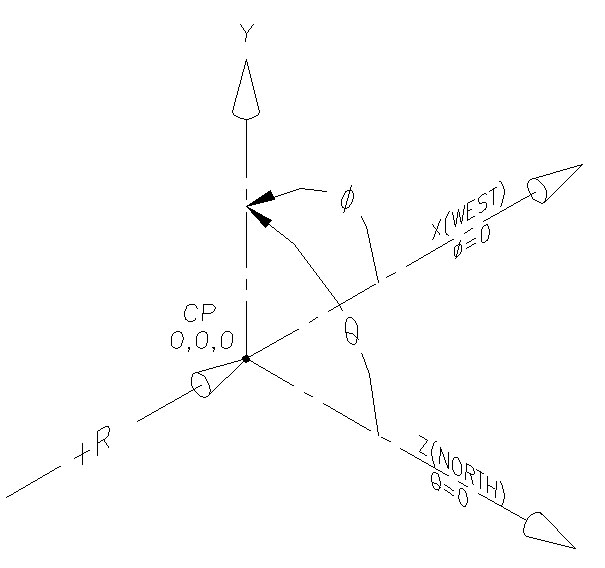
\includegraphics[width=0.7\textwidth]{Figures/coord2.jpg}
    \rule{35em}{0.5pt}
  \caption[PHENIX coordinate system]{PHENIX coordinate system}
  \label{fig:PHENIXcoord}
\end{figure}

The PHENIX coordinate system in Cartesian coordinates is defines the beam line as the z-axis with the north side of the detector being the positive going direction, due west being the positive going x-axis, and straight up being the positive going y-axis. For spherical coordinates, the azimuthal angle $\phi$ spans $2\pi$ about the z axis with $\phi=0$ pointing due west, i.e. along the x-axis. The polar angle $\theta$ is often converted to pseudorapidity for analysis. Pseudorapidity ($\eta$), often referred to colloquially as ``rapidity,'' (not to be confused with the true rapidity, $y$) is defined as:

\begin{equation}
\eta = - ln \bigg[ tan \bigg( \frac{\theta}{2} \bigg) \bigg].
\end{equation}

where small values of $\eta$ refer to processes and measurements in the central arms and larger values of $\eta$ refer to the forward muon arm regions.
